\section{Anforderungsanalyse}

\subsubsection{Usability und User Experience}

\begin{concept}{Usability und User Experience}\\
Die drei Säulen der Benutzererfahrung:
\begin{itemize}
    \item \textbf{Usability (Gebrauchstauglichkeit):} Grundlegende Nutzbarkeit des Systems
    \item \textbf{User Experience:} Usability + Desirability (Attraktivität)
    \item \textbf{Customer Experience:} UX + Brand Experience (Markenwahrnehmung)
\end{itemize}
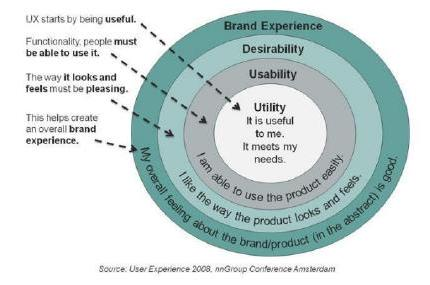
\includegraphics[width=0.9\linewidth]{images/2024_12_29_0d1d7b5551ea1b4b41bdg-02}
\end{concept}

\begin{definition}{Usability-Dimensionen}\\
Die drei Hauptdimensionen der Usability:
\begin{itemize}
    \item \textbf{Effektivität:}
    \begin{itemize}
        \item Vollständige Aufgabenerfüllung
        \item Gewünschte Genauigkeit
    \end{itemize}
    \item \textbf{Effizienz:} Minimaler Aufwand
    \begin{itemize}
        \item Mental
        \item Physisch
        \item Zeitlich
    \end{itemize}
    \item \textbf{Zufriedenheit:}
    \begin{itemize}
        \item Minimum: Keine Verärgerung
        \item Standard: Zufriedenheit
        \item Optimal: Begeisterung
    \end{itemize}
\end{itemize}
\end{definition}

\begin{theorem}{ISO 9241-110: Usability-Anforderungen}\\
Die sieben Grundprinzipien:
\begin{itemize}
    \item Aufgabenangemessenheit
    \item Lernförderlichkeit
    \item Individualisierbarkeit
    \item Erwartungskonformität
    \item Selbstbeschreibungsfähigkeit
    \item Steuerbarkeit
    \item Fehlertoleranz
\end{itemize}
\end{theorem}

\begin{concept}{User-Centered Design (UCD)}\\
Ein iterativer Prozess zur nutzerzentrierten Entwicklung:\\
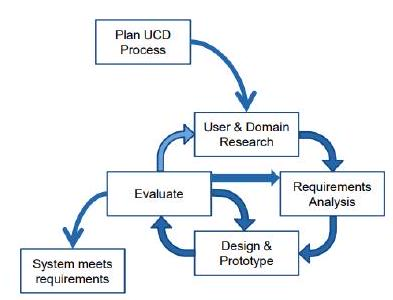
\includegraphics[width=0.6\linewidth]{images/2024_12_29_0d1d7b5551ea1b4b41bdg-03}
\end{concept}
\begin{theorem}{Wichtige Artefakte}
\begin{itemize}
    \item Personas: Repräsentative Nutzerprofile
    \item Usage-Szenarien: Konkrete Anwendungsfälle
    \item Mentales Modell: Nutzerverständnis
    \item Domänenmodell: Fachliches Verständnis
    \item Service Blueprint: Geschäftsprozessmodell
    \item Stakeholder Map: Beteiligte und Betroffene
    \item UI-Artefakte: Skizzen, Wireframes, Designs
\end{itemize}
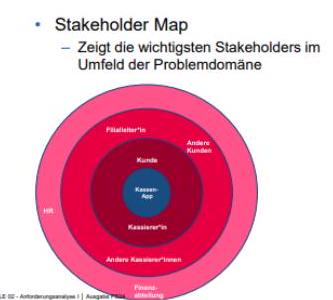
\includegraphics[width=0.5\linewidth]{images/2024_12_29_0d1d7b5551ea1b4b41bdg-04}
\end{theorem}

\subsubsection{Requirements Engineering}

\begin{definition}{Requirements (Anforderungen)}
\begin{itemize}
    \item Leistungsfähigkeiten oder Eigenschaften
    \item Explizit oder implizit
    \item Müssen mit allen Stakeholdern erarbeitet werden
    \item Entwickeln sich während des Projekts
\end{itemize}
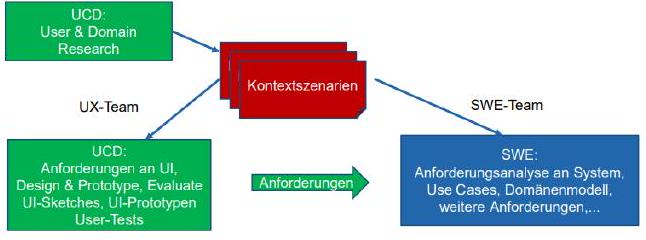
\includegraphics[width=\linewidth]{images/2024_12_29_0d1d7b5551ea1b4b41bdg-04(1)}
\end{definition}

\subsection{Use Cases}

\begin{definition}{Use Case (Anwendungsfall)}\\
Textuelle Beschreibung einer konkreten Interaktion zwischen Akteur und System:
\begin{itemize}
    \item Aus Sicht des Akteurs
    \item Aktiv formuliert
    \item Konkreter Nutzen
    \item Essentieller Stil (Logik statt Implementierung)
\end{itemize}
\end{definition}

\begin{theorem}{Akteure in Use Cases}
\begin{itemize}
    \item \textbf{Primärakteur:} Initiiert den Use Case, erhält Hauptnutzen
    \item \textbf{Unterstützender Akteur:} Hilft bei der Durchführung
    \item \textbf{Offstage-Akteur:} Indirekt beteiligter Stakeholder
\end{itemize}
\end{theorem}

\begin{KR}{Use Case Erstellung}\\
Schritte zur Erstellung eines vollständigen Use Cases:
\begin{enumerate}
    \item \textbf{Identifikation:}
    \begin{itemize}
        \item Systemgrenzen definieren
        \item Primärakteure identifizieren
        \item Ziele der Akteure ermitteln
    \end{itemize}
    \item \textbf{Dokumentation:}
    \begin{itemize}
        \item Brief/Casual für erste Analyse
        \item Fully-dressed für wichtige Use Cases
        \item Standardablauf und Erweiterungen
    \end{itemize}
    \item \textbf{Review:}
    \begin{itemize}
        \item Mit Stakeholdern abstimmen
        \item Auf Vollständigkeit prüfen
        \item Konsistenz sicherstellen
    \end{itemize}
\end{enumerate}
\end{KR}

\begin{example2}{Brief Use Case}
\textbf{Verkauf abwickeln}

Kunde kommt mit Waren zur Kasse. Kassier erfasst alle Produkte. System berechnet Gesamtbetrag. Kassier nimmt Zahlung entgegen und gibt ggf. Wechselgeld. System druckt Beleg.
\end{example2}

\begin{example2}{Fully-dressed Use Case}
\textbf{UC: Verkauf abwickeln}
\begin{itemize}
    \item \textbf{Umfang:} Kassensystem
    \item \textbf{Primärakteur:} Kassier
    \item \textbf{Stakeholder:} Kunde (schnelle Abwicklung), Geschäft (korrekte Abrechnung)
    \item \textbf{Vorbedingung:} Kasse ist geöffnet
    \item \textbf{Standardablauf:}
    \begin{enumerate}
        \item Kassier startet neuen Verkauf
        \item System initialisiert neue Transaktion
        \item Kassier erfasst Produkte
        \item System zeigt Zwischensumme
        \item Kassier schliesst Verkauf ab
        \item System zeigt Gesamtbetrag
        \item Kunde bezahlt
        \item System druckt Beleg
    \end{enumerate}
\end{itemize}
\end{example2}

\begin{concept}{Systemsequenzdiagramm (SSD)}\\
Formalisierte Darstellung der System-Interaktionen:
\begin{itemize}
    \item Zeigt Input/Output-Events
    \item Identifiziert Systemoperationen
    \item Basis für API-Design
\end{itemize}
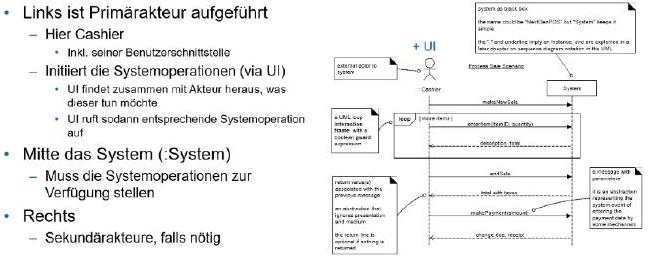
\includegraphics[width=\linewidth]{images/2024_12_29_0d1d7b5551ea1b4b41bdg-06}
\end{concept}

\begin{KR}{SSD Erstellung}
\begin{enumerate}
    \item Use Case als Grundlage wählen
    \item Akteur und System identifizieren
    \item Methodenaufrufe definieren:
    \begin{itemize}
        \item Namen aussagekräftig wählen
        \item Parameter festlegen
        \item Rückgabewerte bestimmen
    \end{itemize}
    \item Zeitliche Abfolge modellieren
    \item Optional: Externe Systeme einbinden
\end{enumerate}
\end{KR}

\begin{example}
\textbf{Aufgabe:} Erstellen Sie einen fully-dressed Use Case für ein Online-Bibliothekssystem. Fokus: "Buch ausleihen"

\textbf{Lösung:}
\begin{itemize}
    \item \textbf{Umfang:} Online-Bibliothekssystem
    \item \textbf{Primärakteur:} Bibliotheksnutzer
    \item \textbf{Stakeholder:} 
    \begin{itemize}
        \item Bibliotheksnutzer: Möchte Buch einfach ausleihen
        \item Bibliothek: Korrekte Erfassung der Ausleihe
    \end{itemize}
    \item \textbf{Vorbedingung:} Nutzer ist eingeloggt
    \item \textbf{Standardablauf:}
    \begin{enumerate}
        \item Nutzer sucht Buch
        \item System zeigt Verfügbarkeit
        \item Nutzer wählt Ausleihe
        \item System prüft Ausleihberechtigung
        \item System registriert Ausleihe
        \item System zeigt Bestätigung
    \end{enumerate}
    \item \textbf{Erweiterungen:}
    \begin{itemize}
        \item 2a: Buch nicht verfügbar
        \item 4a: Keine Ausleihberechtigung
    \end{itemize}
\end{itemize}
\end{example}
